\documentclass{article}
\usepackage[utf8]{inputenc}
\usepackage{graphicx}
\usepackage{listings}

\title{Lab 2}
\author{Hannah Atmer and Xiaoyue Chen \\ Team 6}
\date{October 2021}

\begin{document}

\maketitle

\section{Performance Estimates}

\begin{figure}[h!t]
    \centering
    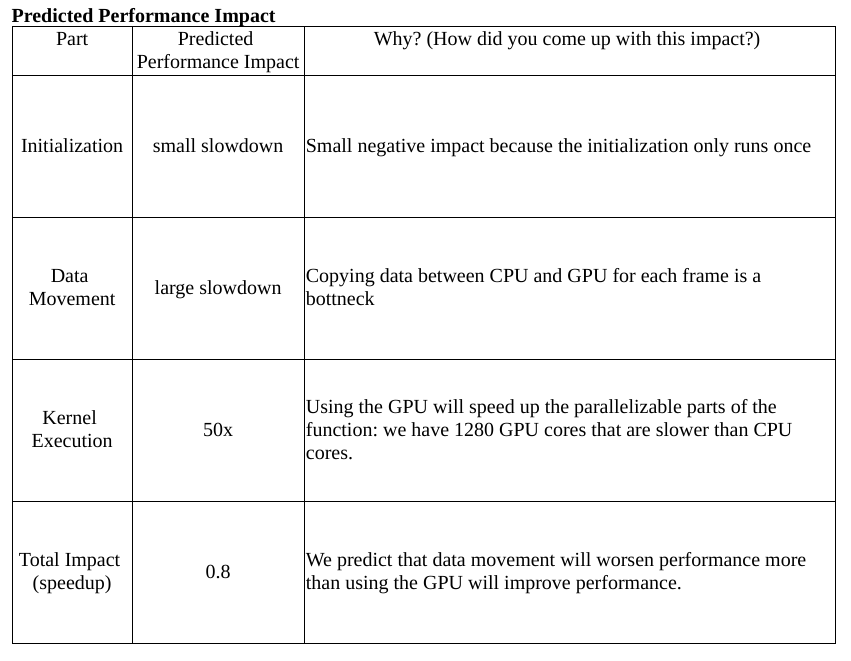
\includegraphics[width=1\textwidth]{predicted.png}
    \caption{Predicted Performance Impact}
    \label{fig:predicted}
\end{figure}

\section{Performance Achieved}

\subsection{Your measured performance results from implementing the optimizations.}

\begin{figure}[h!t]
    \centering
    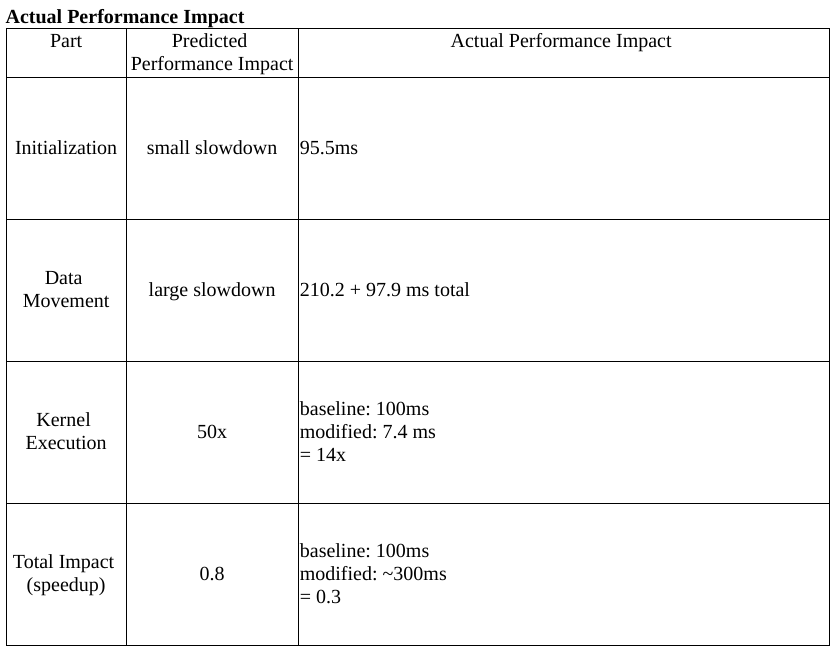
\includegraphics[width=1\textwidth]{actual.png}
    \caption{Actual Performance Impact}
    \label{fig:actual}
\end{figure}

\subsection{The parallel scaling of your implementation.}

\begin{figure}[h!t]
    \centering
    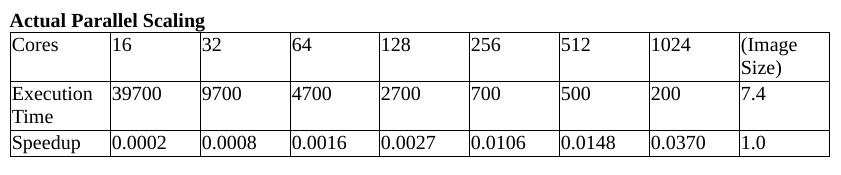
\includegraphics[width=1\textwidth]{parallel.png}
    \caption{Parallel Scaling}
    \label{fig:parallel}
\end{figure}

\section{Discussion}

\subsection{A discussion of the measured results and how they differ from your predictions.}

\subsection{A discussion of what you learned about these optimizations from implementing them and measuring the results.}
We learned that copying the data to and from the GPU took more time than running the code without a GPU. We also learned that it is hard to debug GPU kernel code since the kernel code is compiled at runtime.

\subsection{Comment on any unexpected or odd results.}
Copying data between the CPU and GPU took 300ms total. 200 of these ms were spent copying data from the GPU, meaning that it was half as fast to copy data back from the GPU. 


\subsection{Comments on the difficulty of the GPU offload.}
We used the in-class example, and this worked well except for the lack of informative compiler messages about errors in the kernel code.

\section{Lab comments}

\end{document}
